\documentclass[%
    hyperref={%
        colorlinks,
        linkcolor=sDarkBlue,
        urlcolor=sDarkBlue,
        citecolor=sDarkBlue
    }
]{beamer}
\usetheme{sakura}
\ltjsetparameter{%
    jacharrange={%
        -2, % Exclude Greek and Cyrillic letters.
        -3  % Punctuations and Miscellaneous symbols.
    },
    alxspmode={`/,allow},
    alxspmode={`#,allow},
    alxspmode={92,allow}
}
\usepackage{luatexja-ruby}
\usepackage{arabluatex}
\newfontfamily\arabicfont[%
    Script=Arabic,     % enable ligatures
    RawFeature={%
        +anum,         % use eastern arabic numerals
        +ss05}         % put kasrah below shadda
]{Fira GO Light}
\newfontfamily\translitfont[Ligatures=TeX]{TeX Gyre Termes}
\SetTranslitFont{\translitfont}
\SetTranslitStyle{\itshape}  % \upshape, \itshape
\SetTranslitConvention{dmg}  % dmg, loc, arabica
\usepackage{breakurl}
\usepackage{booktabs}
\usepackage{ccicons}
\usepackage{bxghost}
\usepackage{subcaption}
\usepackage{fontawesome}
\usepackage{amsmath,amssymb}
\usepackage{framed}
\usepackage{listings}
\usepackage[sort]{natbib}
\usepackage{tikz-dependency}
\usepackage{wtref}
\renewcommand{\tablename}{表}
\renewcommand{\figurename}{図}
\newref{tab}
\setrefstyle{tab}{prefix=表}
\newref{fig}
\setrefstyle{fig}{prefix=図}
\newref{math}
\renewcommand{\theequation}{\arabic{equation}}
\newcommand{\inlinecommand}[1]{{\ttfamily #1}}
\setrefstyle{math}{refcmd=(\ref{#1})}
\setbeamertemplate{caption}[numbered]
\setbeamertemplate{caption label separator}{:}
\usetikzlibrary{automata,positioning,arrows,calc}
\defcitealias{poetics}{アリストテレス『詩学』1457b}
\defcitealias{ginga}{宮澤賢治『銀河鉄道の夜』九 ジョバンニの切符}
\DeclareMathOperator{\exponential}{exp}
\newcommand\header[1]{\multicolumn{1}{c}{\textbf{#1}}}
\newenvironment{quoteblock}{%
    \def\FrameCommand{%
        {\color{sLightGray}{\vrule width 3pt}}%
        \hspace{10pt}
    }%
    \MakeFramed {\advance\hsize-\width \FrameRestore}}%
{\endMakeFramed}
\lstset{%
    language={[LaTeX]TeX},
    basicstyle=\ttfamily\footnotesize,
    keywordstyle=\bfseries,
    texcsstyle=*\color{sRed}\bfseries,
    commentstyle=\color{sDarkBlue}
}
\renewcommand\refname{参考文献}
\renewcommand\appendixname{付録}
\title{Lua\TeX{}-jaとbeamerで研究発表用のスライドを作る}
\institute{所属}
\author{著者 太郎}
\date{{\number\year}年{\number\month}月{\number\day}日}
\usepackage{gb4e,cgloss4e}
\renewcommand\eachwordone{\relax}
\renewcommand\eachwordtwo{\itshape}
\renewcommand\eachwordthree{\relax}
\noautomath%
\begin{document}

    \maketitle

    \section{はじめに}
    \begin{frame}
        \frametitle{はじめに}
        このスライドは \faGithub\ \href{https://github.com/pecorarista/sakuratheme}{\ttfamily pecorarista/sakuratheme}のデモとして作ったものです.

        \bigskip

        そのため作り方を詳しく説明することはしませんが,
        コードはすべて上記のレポジトリに含まれているので気になる方は参照ください.
        \bigskip

        また言語学関連の話題の\LaTeX における扱い方を網羅的に知りたい方は
        \href{https://www1.essex.ac.uk/linguistics/external/clmt/latex4ling/}
        {LaTeX for Linguists}が参考になります.
    \end{frame}

    \section{基本}
    \begin{frame}
        \frametitle{表の挿入}
        Beamerでは論文などの表のソースコードをほぼそのまま利用できて便利です.
        \begin{table}
            \centering
            \caption{表の例.}\tablabel{tab}
            \begin{tabular}{rrr}
                \toprule
                \header{a} & \header{b} & \header{c} \\
                \midrule
                0.123 & 0.28  & 0.32 \\
                0.234 & 1.25  & 0.45 \\
                0.123 & 0.28  & 0.32 \\
                0.234 & 1.25  & 0.45 \\
                \bottomrule
            \end{tabular}
        \end{table}
    \end{frame}

    \begin{frame}
        \frametitle{数式}
        以下で定義される関数$\sigma$を\emph{logistic sigmoid}関数と呼ぶ\citep{prml}.
        \begin{align}
            \sigma(\mu) = \frac{1}{1 + \exponential(-\mu)} \mathlabel{sigmoid}
        \end{align}
        数式を参照することもできます\mathref{sigmoid}.
    \end{frame}

    \begin{frame}[fragile]
        \frametitle{画像の引用}
        画像の挿入には\inlinecommand{\textbackslash includegraphics}コマンドを使います.
        Creative Commonsライセンスの作品には\href{https://ctan.org/pkg/ccicons}{\texttt{ccicons}}パッケージのアイコンを利用すると便利です.
        必要に応じて\inlinecommand{\textbackslash href\{{\rmfamily\mdseries\itshape uri}\}\{{\rmfamily\mdseries\itshape text}\}}で元のファイルへリンクを張ります.

        \bigskip

        \begin{figure}
            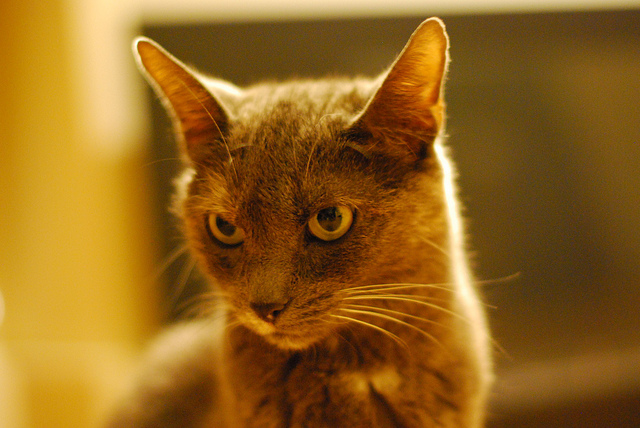
\includegraphics[width=0.4\textwidth]{cat.jpg}
            \caption{\href{https://www.flickr.com/photos/selda_eigler/8687127864/in/photolist-eeDNsC-qWFs4R-7CNDjJ-9c8DxY-eeDNhC-UCZ63T-dJNGUc-e5Nk39-988EVA-kUgwo-owDcVP-jQGjjt-5zkGTy-7WRCUo-b91XbZ-Mj8Ku-5pzwSA-9Bct2H-7CNHMY-7CJJMB-8MyEYn-9x45Mp-7JTq8M-ZrpGJ9-8fRht4-4SxVZT-5pzwjJ-ZsPJjL-aE44GL-dF6uWD-kqbHgM-5F373J-ZsQrVG-qyD7E9-ajyDPL-4WDvTp-KbDSc-5kCxD9-4MdeUo-pgDQcG-pPWrXD-662AFD-oTnC8k-apYceQ-nJSaaY-7CJLZv-7CJJMn-7CNFsU-XNMWkw-ccdtT9}{\emph{Cat} by Selda Eigler} \ccby.}
        \end{figure}

    \end{frame}

    \begin{frame}
        \frametitle{長め文章の引用}
        \href{https://ctan.org/pkg/framed}{\texttt{framed}}パッケージの\inlinecommand{leftbar}環境を使うと引用であることが分かりやすくなります.

        \begin{quoteblock}
    ἅπαν δὲ ὄνομά ἐστιν ἢ κύριον ἢ γλῶττα ἢ μεταφορὰ ἢ κόσμος ἢ πεποιημένον ἢ ἐπεκτεταμένον ἢ ὑφῃρημένον ἢ ἐξηλλαγμένον.

    \hfill \citetalias{poetics}
        \end{quoteblock}

        \begin{quoteblock}
            「あの森\ruby{琴}{ライラ}の宿でせう。
            あたしきつとあの森の中には、
            むかしの大きなオーケストラの人たちが集まつていらつしやると思ふわ。
            まはりには青い孔雀やなんかたくさんゐると思ふわ。」
            女の子が答へました。

            \hfill \citetalias{ginga}
        \end{quoteblock}
    \end{frame}


    \section{言語学}
    \subsection{グロス}
    \begin{frame}[fragile]
        \frametitle{グロスI}
        \href{https://ctan.org/pkg/gb4e}{\texttt{gb4e}}と
        \href{https://ctan.org/pkg/gb4e}{\texttt{cgloss4e}}パッケージを利用します.

        \bigskip

        1行目に正書法の表記を使い,
        2行目にイタリックでラテン字転写する場合はプリアンブルに以下のような記述をします.

        \begin{leftbar}
        \begin{lstlisting}[%
            language={[LaTeX]TeX},
            % asterisk for highlight backslash
            moretexcs={@ifundefined,eachwordone,eachwordtwo,eachwordthree,noautomath}
        ]
\usepackage{gb4e,cgloss4e}
\renewcommand\eachwordone{\relax}
\renewcommand\eachwordtwo{\itshape}
\renewcommand\eachwordthree{\relax}
\noautomath
        \end{lstlisting}
        \end{leftbar}
    \end{frame}

    \begin{frame}[fragile]
        \setlength{\glossglue}{5pt plus 2pt minus 1pt}\footnotesize
        \frametitle{グロスII}
        余白が狭く感じる場合は以下のように調整を行うとよいです.
        \begin{leftbar}
        \begin{lstlisting}[%
            language={[LaTeX]TeX},
            moretexcs={setlength,glossglue},
            morekeywords={plus,minus}
        ]
\setlength{\glossglue}{5pt plus 2pt minus 1pt}
        \end{lstlisting}
    \end{leftbar}

        結果はこのようになります.
        \begin{exe}
            \ex%
            \glll%
            {これは} {ロシア語の} {教科書} {です} \\
            {kore-wa} {rosia-go-no} {kyōkašo} {desu} \\
            {this-\textsc{top}} {Russia-language-\textsc{gen}} {textbook} {be} \\
            \trans%
            ``This is a textbook of the Russian language''
            \ex%
            \glll%
            {Это} {учебник} {русского} {языка} \\
            % {Э'то} {уче'бник} {ру'сского} {языка'} \\
            {èto} {učebnik} {russk-ovo} {jazyk-a} \\
            {this} {textbook.\textsc{sg.nom}} {Russian-\textsc{m.sg.gen}} {language-\textsc{gen}} \\
            \trans%
            ``This is a textbook of the Russian language.''
        \end{exe}
    \end{frame}

    \subsection{アラビア文字}
    \begin{frame}[fragile]
    \frametitle{アラビア文字I}
        もしアラビア文字を入力したければ\href{https://ctan.org/pkg/arabluatex?lang=en}{arabluatex}の利用をおすすめします.
    \begin{leftbar}
    \begin{lstlisting}[%
        language={[LaTeX]TeX},
        % asterisk for highlight backslash
        moretexcs={
            ltjsetparameter,
            arabicfont,
            newfontfamily,
            translitfont,
            SetTranslitFont,
            SetTranslitStyle,
            SetTranslitConvention
        },
        morekeywords={},
    ]
\usepackage{arabluatex}
\newfontfamily\arabicfont[%
  Script=Arabic, % enable ligatures
  RawFeature={%
    +anum, % use eastern arabic numerals
    +ss05} % put kasrah below shadda
]{Fira GO}
\newfontfamily\translitfont[Ligatures=TeX]{%
  TeX Gyre Termes
}
\SetTranslitFont{\translitfont}
\SetTranslitStyle{\itshape} % \upshape, \itshape
\SetTranslitConvention{arabica} % dmg, loc, arabica
    \end{lstlisting}
    \end{leftbar}
    \end{frame}

    \begin{frame}[fragile]
        \frametitle{アラビア文字II}
        ラテン文字で入力できるのでRTL(右から左への横書き)や合字に対応していないエディタでも編集できます.
        転写の方法は\inlinecommand{dmg}, \inlinecommand{arabica}, \inlinecommand{loc}の3種類から選べます.

        \begin{leftbar}
        \begin{lstlisting}[%
            language={[LaTeX]TeX},
            % asterisk for highlight backslash
            moretexcs={arb},
            morekeywords={arab}
        ]
\begin{arab}[fullvoc]
    'anta tatakallamu 'l-lu.gaTa
    'l-`arabiyyaTa jayyidaN!
\end{arab}
\arb[trans]{'anta tatakallamu
            'l-lu.gaTa 'l-`arabiyyaTa jayyidaN!}
        \end{lstlisting}
        \end{leftbar}

        \begin{arab}[fullvoc]
            'anta tatakallamu 'l-lu.gaTa 'l-`arabiyyaTa jayyidaN!
        \end{arab}

        \bigskip

        \arb[trans]{'anta tatakallamu 'l-lu.gaTa 'l-`arabiyyaTa jayyidaN!}
    \end{frame}

    \begin{frame}
        \frametitle{係り受け解析}
        係り受けの図を挿入するには\href{https://ctan.org/pkg/tikz-dependency}{\texttt{tikz-dependency}}を利用します.

        \bigskip

        \begin{figure}
            \begin{subfigure}[t]{0.38\textwidth}
                \centering
                \scalebox{.9}{%
                    \begin{dependency}[hide label]
                        \begin{deptext}[column sep=2\zw]
                            兵庫を \& 訪れた。 \\
                        \end{deptext}
                        \depedge{2}{1}{目的語}
                    \end{dependency}
                }
                \caption{文節単位・ラベルなし}\figlabel{dep-without-labels}
            \end{subfigure}
            \begin{subfigure}[t]{0.6\textwidth}
                \centering
                \scalebox{.9}{%
                    \begin{dependency}[text only label,label style={above}]
                        \begin{deptext}[column sep=2\zw]
                            兵庫  \& を  \& 訪れ \& た。 \\
                            {\scriptsize 固有名詞} \& {\scriptsize 接置詞} \& {\scriptsize 動詞} \& {\scriptsize 助動詞} \\
                        \end{deptext}
                        \depedge{1}{2}{格表示}
                        \depedge{3}{1}{目的語}
                        \depedge{3}{4}{助動詞}
                    \end{dependency}
                }
                \caption{単語単位・ラベルあり}\figlabel{dep-with-labels}
            \end{subfigure}
            \caption{文「兵庫を訪れた。」を係り受け解析し,図示したもの.}
        \end{figure}
        \figref{dep-without-labels}や\figref{dep-with-labels}のように参照することができます.
    \end{frame}

    \begin{frame}
        \frametitle{その他}
        箇条書きの項目が鉤括弧から始まるときの注意点
        \begin{itemize}
            \item こんにちは
            \item 「こんにちは」

                行頭の余白が大きい
            \item \leavevmode\inhibitglue 「こんにちは」

                \texttt{\textbackslash item \textbackslash leavevmode\textbackslash inhibitglue} で余白を調整
        \end{itemize}

        \bigskip

        参照:\href{http://doratex.hatenablog.jp/entry/20140714/1405302796}{「TeX Live 2014のpTeX系列における\textbackslash inhibitglueの仕様変更」}
    \end{frame}

    \begin{frame}[plain,noframenumbering,allowframebreaks]
        \frametitle{参考文献}
        \small
        \bibliographystyle{jecon}
        \bibliography{demo}
    \end{frame}

\end{document}
